\subsection{Photo Measures}

\subsubsection{Vorstellung}
Die App \emph{Photo Measures} von \emph{Big Blue Pixel Inc.} hat zur Zeit des Downloads (20. Januar 2018) bei insgesamt 425 abgegeben Bewertungen eine durchschnittliche Bewertung von 4,3 von 5 Sternen im Google Play-Store \citep{PixelPM}.
Auch diese App wird wie die beiden zuvor vorgestellten Apps unter der Kategorie ``Effizienz'' gelistet.
Im Gegensatz zu den anderen Apps ist diese jedoch nicht kostenlos erhältlich, sondern kann für einen Preis von 3,99 Euro erworben werden. \todo{kaufen?} 
Die Beschreibung im Play-Store selbst lautet wie folgt \todo{cite aus playstore}:

\begin{quote}
  ``Photo Measures is the best and easiest way to save measures on your own photos on Android.''
\end{quote}

\noindent
Beim ersten Start der App wird der Nutzer über eine Textbox, welche auf ein Plus-Symbol (siehe \autoref{fig:pmmenu}) mit der Unterschrift ``New'' zeigt, auf die möglichen Aktionen hingewiesen, die er in diesem Appzustand ausführen kann.

\begin{figure}[h]
  \centering
	\begin{subfigure}[t]{0.4\textwidth}
		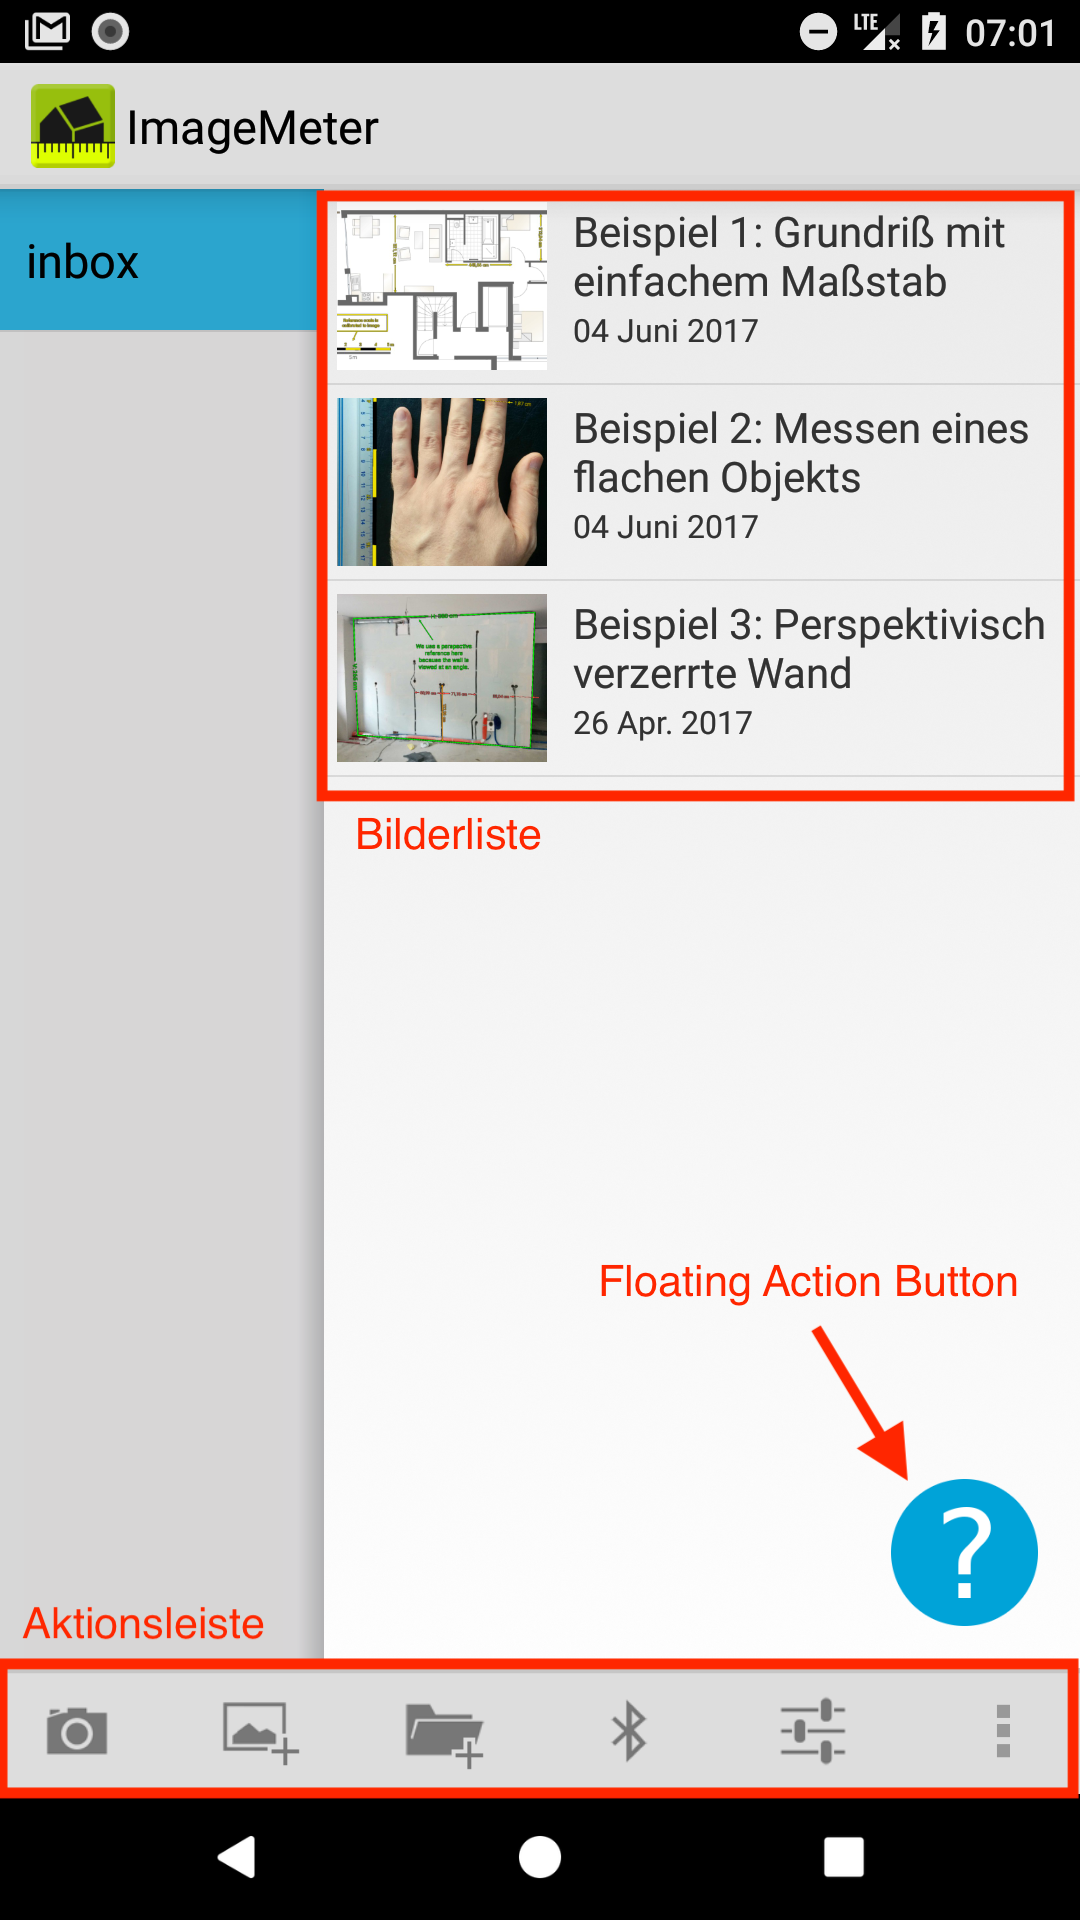
\includegraphics[keepaspectratio, width=\textwidth]{photo_measures/menu}
		\caption{Startbildschirm}
		\label{fig:pmmenu}	
	\end{subfigure}
	\begin{subfigure}[t]{0.4\textwidth}
		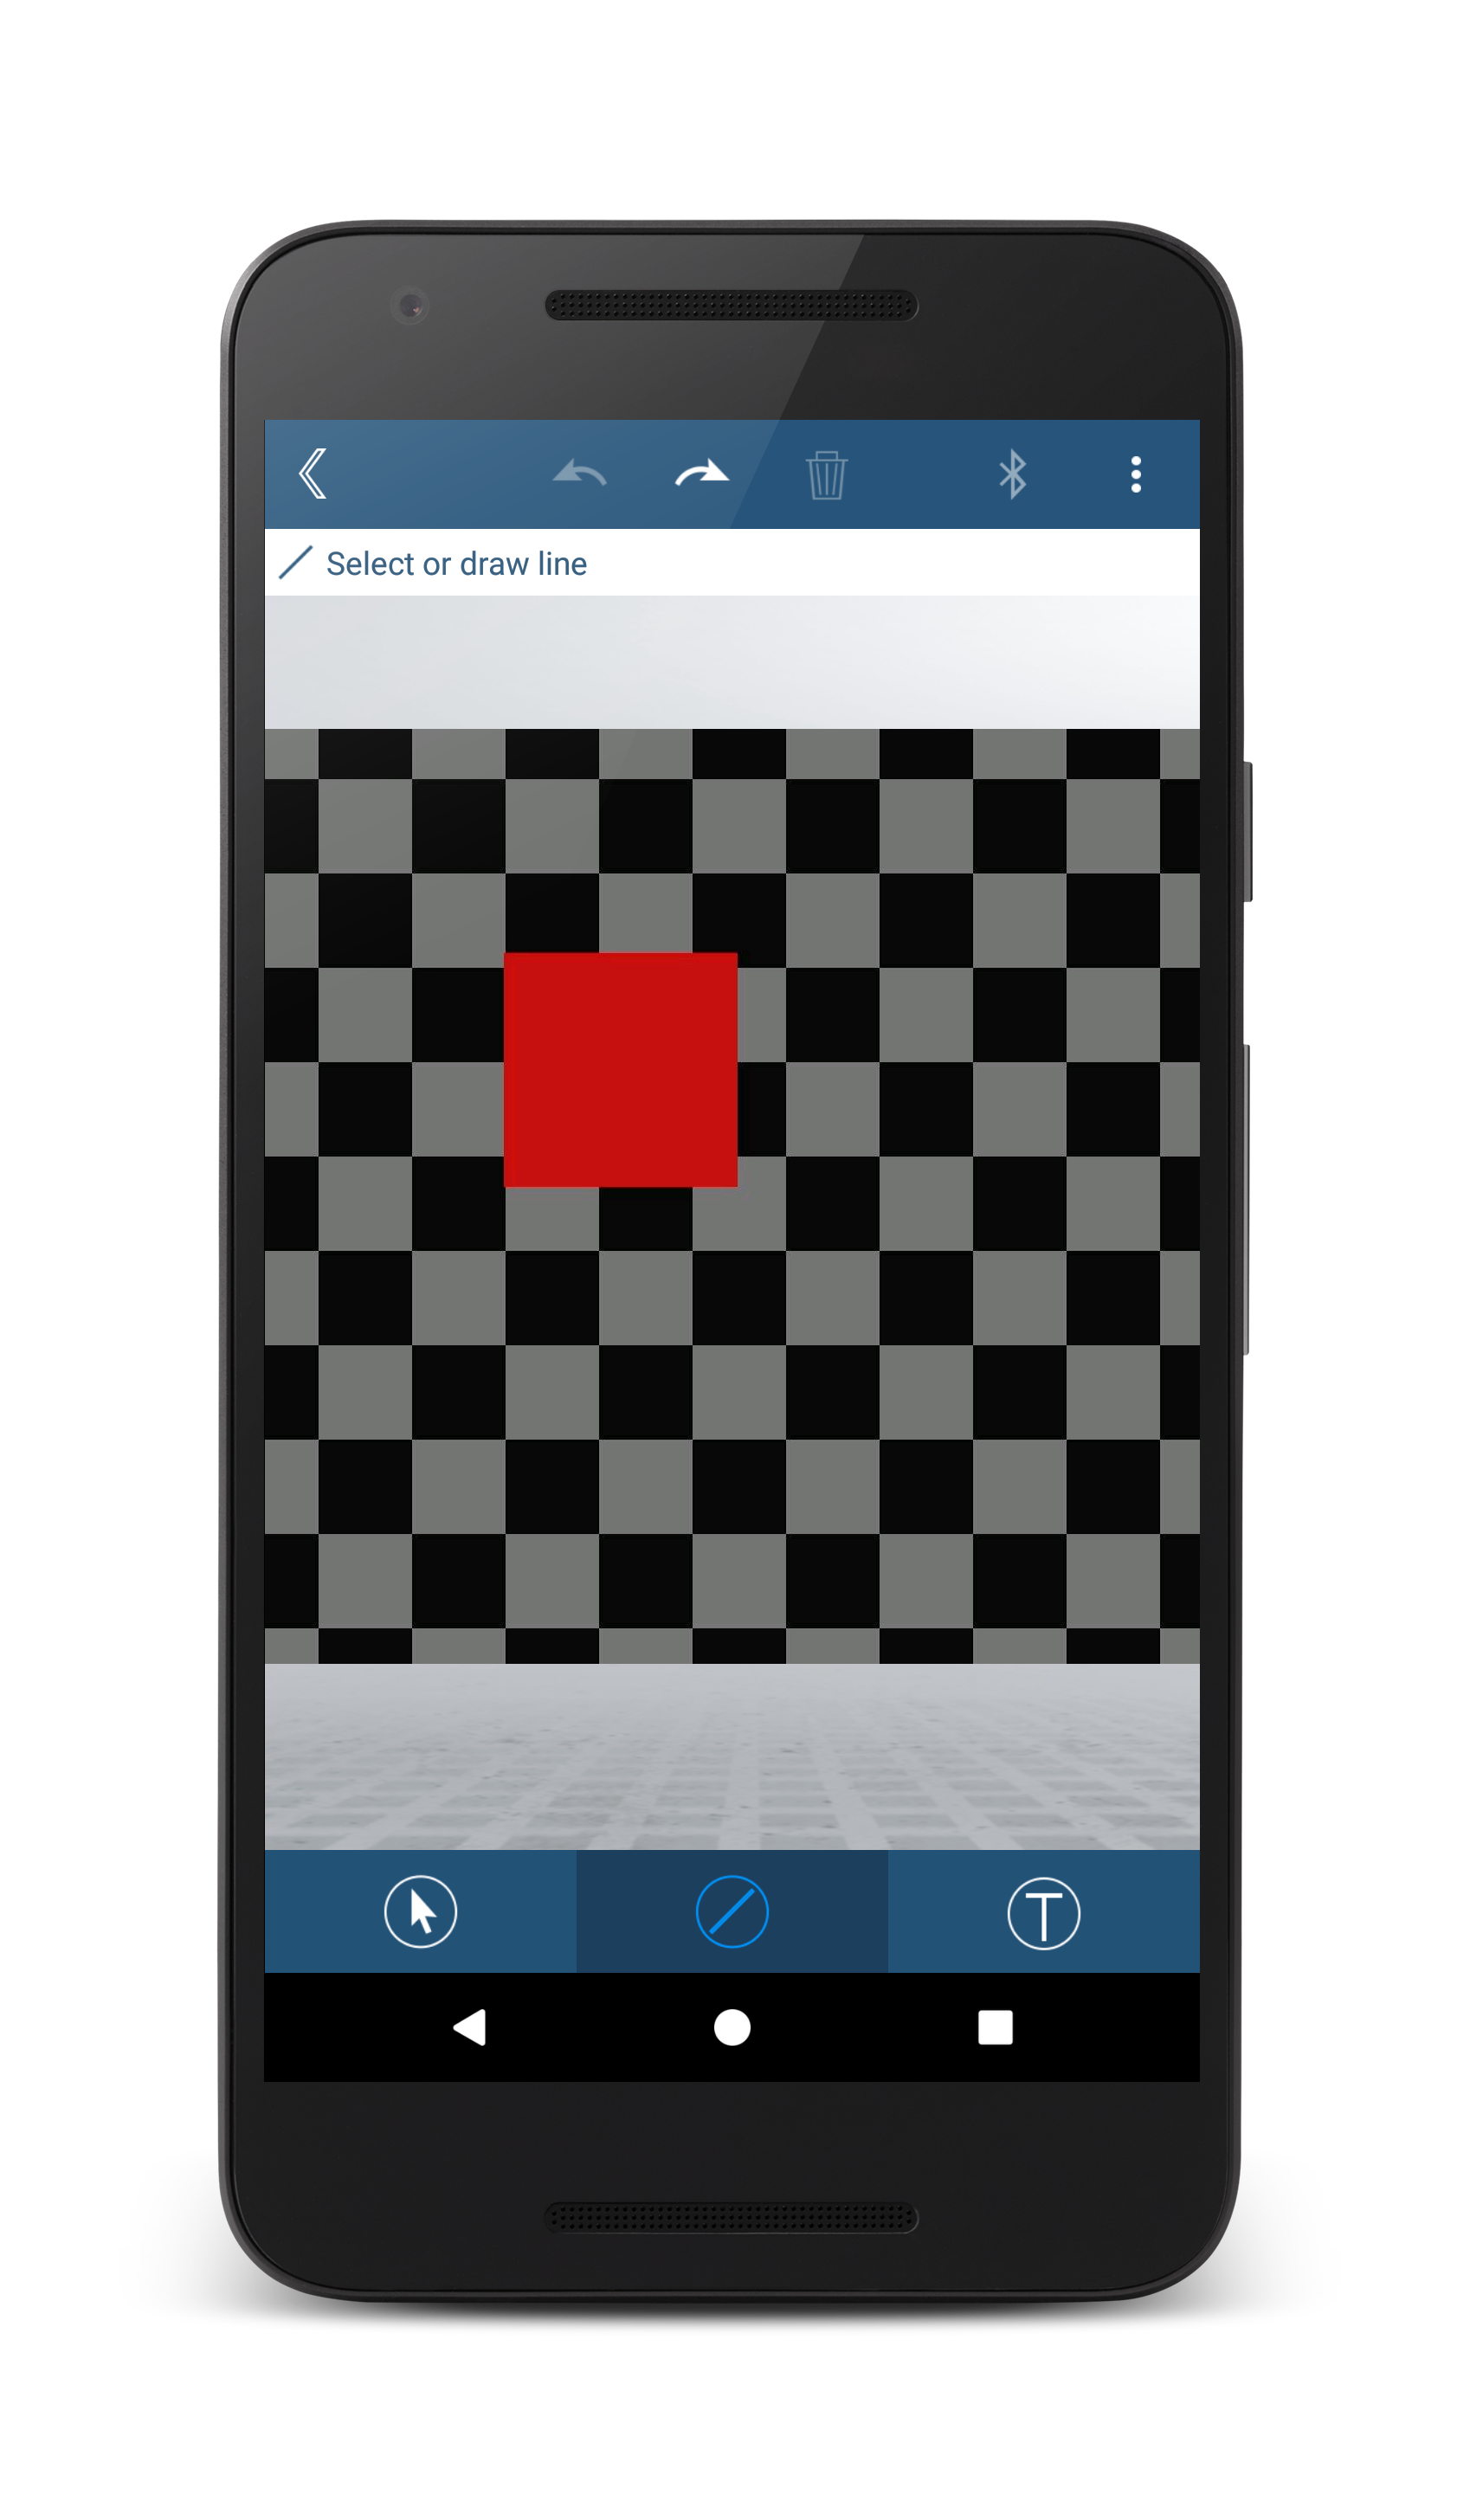
\includegraphics[keepaspectratio, width=\textwidth]{photo_measures/help}
		\caption{Hilfe-Overlay beim initialen Start der Aufmaß-Funktion} 
		\label{fig:pmhelp}	
	\end{subfigure}
  \caption{Measure \& Sketch beim Start der App und in der Aufmaß-Funktion}
\end{figure}

\noindent
Durch einen Klick auf das beschriebene Plus-Symbol öffnet sich ein Dialog, der den Benutzer auffordert, ein Bild auszuwählen.
Hierzu kann der Benutzer das Bild direkt aus der Galerie importieren, oder ein Neues mit der Kamera aufnehmen. \\
Anschließend wechselt die App in eine andere Benutzeroberfläche, in der das ausgewählte Bild und eine Statusleiste am unteren Rand des Bildschirms zu sehen sind (\autoref{fig:pmhelp}).
Wenn der Benutzer diese Oberfläche zum ersten Mal öffnet, zeigt die App außerdem ein Hilfe-Overlay, welches dem Benutzer darüber informiert, wie Formen in das Bild eingezeichnet werden können.  \\

Zudem werden nur die Funktionen, die zum jeweiligen Systemzustand ausführbar sind (z.B. Farbe ändern nur wenn Form ausgewählt), in der Statusleiste am unteren Bildschirmrand angezeigt.
Die Statusleiste bietet, wenn keine Form ausgewählt ist, die Möglichkeit zwischen drei verschienden Formen (Linie, Winkel, Freitext) zu wählen, die gewünschte Größe einzustellen, oder das Bild schrittweise um 90 Grad im Uhrzeigersinn zu drehen.
Wenn eine Form ausgewählt ist, kann diese über die Statusleite im Nachhinein beschriftet, gefärbt oder gelöscht werden. \\

Auch in dieser App lassen sich gespeicherte Bilder zu einem späteren Zeitpunkt weiter bearbeiten.
Außerdem können mehrere Bilder gleichzeitig zusammen in einer \emph{PDF} oder als jeweils als einzelnes Bild geteilt werden.

\subsubsection{Evaluation}
Die App zeigt beim ersten Start ein helfendes Overlay, welches dem Nutzer genau erklärt, wie die App zu benutzen ist. Dieser Punkt fällt nach Nielsen unter \ref{itm:10} (Siehe Abbildung\ref{fig:pmhelp}) \\
 
Aktionen sind nur dann verfügbar, wenn sie benutzbar sind. Somit werden Fehler vorgebeugt, und der Benutzer weiß zu jeder Zeit, in welchem Systemzustand er sich befindet. Dies korrespondiert zu den Heuristiken~\ref{itm:1} und \ref{itm:5}. \todo{2 bilder mit bottom-bars} \\

Die App bedient sich einer Reihe universell bekannter Icons, sodass intuitiv erkennbar ist, welche Aktion sich hinter welchem Button verbirgt, ohne groß darüber nachdenken zu müssen. Zusätzlich stehen die entsprechenden Aktionen als Text unter den Icons. Dies kann nützlich sein, wenn ein Icon nicht auf Anhieb wiedererkannt wird. \ref{itm:4} \todo{ref auf pic von bottom-bars} \\

Des Weiteren gibt die App dem Benutzer die Möglichkeit, Formen, Größen und Farben anzupassen. Dies fördert eine flexible und effizente Benutzung. \ref{itm:7} \\

Ein durchaus schwerwiegender negativer Punkt liegt bei der Benutzerkontrolle \ref{itm:3} der App. So ist es dem Benutzer nicht möglich, über einen Undo- bzw. Redo-Button seine Aktionen zu revidieren. Dies ist gerade bei der Bearbeitung von Bildern, wo es viele aneinandergereihte Aktionen des Benutzers gibt, eine entscheidende Funktionalität, welche nicht nur die Gedächtnisbelastung des Benutzer senken, sondern auch den ``Joy of Use'' deutlich steigern kann. \\

Zudem bietet die App keine für den Nutzer erkennbare Ausstiegsmöglichkeit \ref{itm:6} an. Es gibt weder einen Zurück-Button, noch einen Button um das annotierte Bild explizit zu speichern. Die einzige Ausstiegsmöglichkeit erfolgt über die Zurück-Navigationstaste des Smartphones, welche das Bild auch zusätzlich speichert. Diese Lösungsvariante ist für den Nutzer nicht intuitiv verständlich. \todo{bild}

Die App erfüllt nahezu alle acht (\ref{itm:11}-\ref{itm:18}) Heuristiken für mobile Geräte. Zu jeder Zeit ist auf dem Bildschirm erkennbar, welche Form zur Zeit ausgewählt ist. Das Smartphone kann während der Benutzung pausiert bzw. gedreht werden, ohne dass Informationen verloren gehen, oder der Benutzer durch unbekannte Bausteine überrascht wird. \todo{screens} Hier fällt als einziger negativer Punkt die unzureichende Gesten-Unterstützung auf \ref{itm:13}. So malt der Benutzer unabsichtlich mit jeder Zoom-Geste eine Form in das Bild, welche danach wieder gelöscht werden muss, da es keine Undo-Funktion gibt. \\

